

\section{Metric analysis}\label{sec:graphcentrality}

To demonstrate the information provided by different centrality metrics, a simple intuitive network (the co-author network in \autoref{fig:authorgroup}) shall be used. This subsection will access the efficiency of graph centrality metrics in their ability to identify important nodes within a network. 


\subsection{Degree Centrality}
The simplest, and most intuitive, metric is degree centrality \citep{degreefreeman}. This is described as the sum of all links incident on a node - simply put, we count the number of edges going in and out of a node. This gives us an idea of the importance of a node and has been used to calculate influence within social media or the probability of a profile committing online auction fraud \citep{degreetwitter,degreefreeman}.

For the author network, \autoref{fig:degauth} we see that many of the names on the list are either contributors to the MCM or have worked with them at Leeds. It is also seen that the authors with the most collaborations, or links, are very likely to appear within the most cited or citing papers (\autoref{tab:In-Degree_Citation} and \autoref{tab:Out-Degree_Citation} discussed below). This is likely because both development (well-cited) and the evaluation/usage (well citing) of a mechanism requires knowledge from a range of different fields, making it an interactively collaborative process. 

\begin{figure}[H]
     \centering
         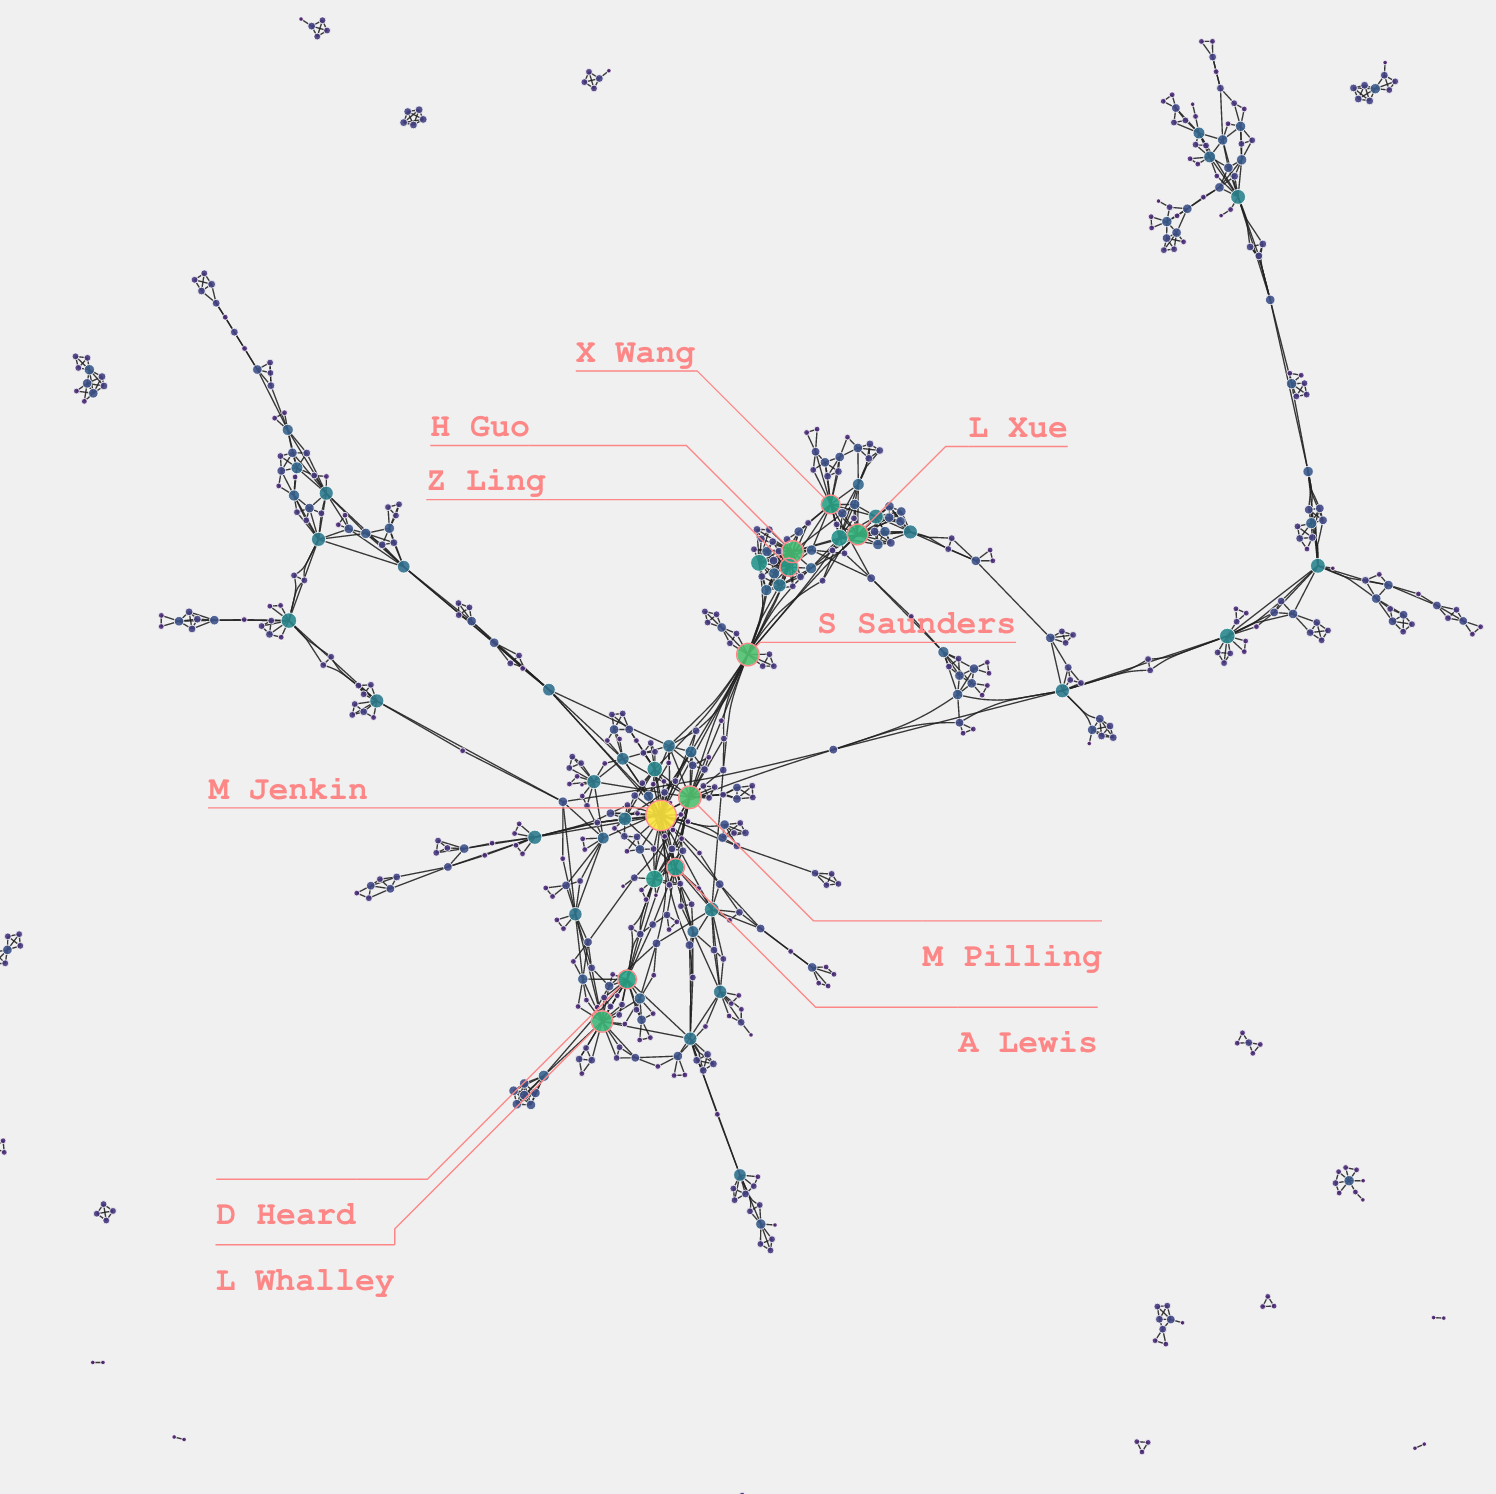
\includegraphics[width=.8\textwidth]{figures_c3/degreeauthor.png}
         \begin{table}[H] \centering\begin{tabular}{lr}
\toprule
   \hphantom{ } M Jenkin &  39 \\
 \hphantom{ } S Saunders &  25 \\
  \hphantom{ } M Pilling &  25 \\
      \hphantom{ } H Guo &  24 \\
  \hphantom{ } L Whalley &  23 \\
      \hphantom{ } L Xue &  22 \\
    \hphantom{ } D Heard &  19 \\
     \hphantom{ } X Wang &  19 \\
     \hphantom{ } Z Ling &  18 \\
    \hphantom{ } A Lewis &  17 \\
\bottomrule
\end{tabular}
    \label{tab:degree_Author}
    % \caption{\textbf{Author network}: Top 10 ranked items using degree centrality}
    \end{table}

    
        \caption{ \textbf{Degree Centrality.} In applying the degree centrality to the co-authorship network, it is possible to pick the authors with the greatest number of papers, of which the top 10 have been listed.}
        \label{fig:degauth}
\end{figure}

% \begin{table}[H]
     \begin{tabular}{p{0.5\textwidth}p{0.35\textwidth}c}
     \toprule
      & & \\\\
     Protocol for the development of the Master Chemical Mechanism, MCM v3 Part A tropospheric degradation of nonaromatic volatile organic compounds & \cite{degree0} & 291  \\ \\
        Protocol for the development of the Master Chemical Mechanism, MCM v3 Part B tropospheric degradation of aromatic volatile organic compounds & \cite{degree1} & 174  \\ \\
        Development of a detailed chemical mechanism MCMv3. 1 for the atmospheric oxidation of aromatic hydrocarbons & \cite{degree2} & 103  \\ \\
        Atmospheric oxidation capacity sustained by a tropical forest & \cite{degree3} & 60  \\ \\
        Photochemical ozone creation potentials for organic compounds in northwest Europe calculated with a master chemical mechanism & \cite{degree4} & 54  \\ \\
        \bottomrule
    \end{tabular}
    \label{tab:degree_Citation}
    \caption{\textbf{Citation network}: Top 5 ranked items using degree centrality}
    \end{table}

    
% \begin{table}[H]
     \begin{tabular}{p{0.5\textwidth}p{0.35\textwidth}c}
     \toprule
      & & \\\\
     Protocol for the development of the Master Chemical Mechanism, MCM v3 Part A tropospheric degradation of nonaromatic volatile organic compounds & \cite{degree0} & 340  \\ \\
        Protocol for the development of the Master Chemical Mechanism, MCM v3 Part B tropospheric degradation of aromatic volatile organic compounds & \cite{degree1} & 250  \\ \\
        Atmospheric oxidation capacity sustained by a tropical forest & \cite{degree2} & 187  \\ \\
        Development of a detailed chemical mechanism MCMv3. 1 for the atmospheric oxidation of aromatic hydrocarbons & \cite{degree3} & 184  \\ \\
        HO x radical regeneration in the oxidation of isoprene & \cite{degree4} & 176  \\ \\
        \bottomrule
    \end{tabular}
    \label{tab:degree_Co-Citation}
    \caption{\textbf{Co-Citation network}: Top 5 ranked items using degree centrality}
    \end{table}

    

\subsubsection*{Directed Degree}
For graphs where link direction holds an inherent meaning regarding their representation (for example in the citation graph an outward link symbolises that paper citing the one that the link points to), it is possible to further divide the degree centrality metric into inwards and outward links. This can allow us to separate items which provide a large number of lots of information (in-degree) and those who collate or collect it (out-degree). In applying these metrics to the directed citation graph, it is possible to get an insight into the core MCM development papers (\autoref{tab:In-Degree_Citation}) and separtate them from those which make use of the mechanism as part of a greater study (\autoref{tab:Out-Degree_Citation}).



% \paragraph{In-Degree}
\begin{table}[H]
    \centering
     \begin{tabular}{p{0.6\textwidth}r}
     \toprule
      & \\ \\
     Protocol for the development of the Master Chemical Mechanism, MCM v3 Part A tropospheric degradation of nonaromatic volatile organic compounds & \cite{mcmpartA}   \\ \\
        Protocol for the development of the Master Chemical Mechanism, MCM v3 Part B tropospheric degradation of aromatic volatile organic compounds & \cite{mcmpartB}   \\ \\
        Development of a detailed chemical mechanism MCMv3. 1 for the atmospheric oxidation of aromatic hydrocarbons & \cite{detailedmcm}   \\ \\
        \bottomrule
    \end{tabular}
    \caption{\textbf{In-Degree of the citation network}: The top 3 most cited papers.}
    \label{tab:In-Degree_Citation}
    \end{table}

    

% \paragraph{Out-Degree}
\begin{table}[H]
    \centering
     \begin{tabular}{p{0.6\textwidth}r}
     \toprule
      & \\ \\
     The MCM v3.3.1 degradation scheme for isoprene & \cite{isopmcm}  \\ \\
        Atmospheric photochemical reactivity and ozone production at two sites in Hong Kong Application of a master chemical mechanismphotochemical box model & \cite{hongkongmcm}   \\ \\
        HOx budgets during HOxComp A case study of HOx chemistry under NOxlimited conditions & \cite{hoxcompmcm}  \\ \\
        \bottomrule
    \end{tabular}
    \caption{\textbf{Out-Degree of the citation network}: The top 3 most citing papers.}
    \label{tab:Out-Degree_Citation}
    \end{table}

    


\subsection{Closness Centrality}
Often within a network, we are interested in how easy it is to to get information from one node to every other node. This is what the closeness centrality tells us. To calculate a nodes closeness we begin by taking the reciprocal sum of all the Dijkstra paths\footnote{The shortest available path.} to every other node \citep{closeness-book,closeness}. 
This gives is a representation of how far information from a certain will need to travel to reach every other node. Such a metric has applications in intelligence gathering, telecommunications and word importance within key-phrase extraction \citep{terror,examples_centrality,phrase}.

\begin{quote}
\textit{
\textbf{Example analogy:} If we take the UK rail network as an example, York station will have a high closeness value as it is well connected and central in location. This means it is easy to reach every other location when compared to other stations.
}
\end{quote}

For the co-authorship network, \autoref{fig:closeauth}, nodes have been coloured by their closeness value. Here a heat-map-like effect may be observed, showing that information between the dense Leeds-York cluster is easier to disseminate across all parts of the graph than that of localised branches of authors less involved with the development team. The results of the closeness centrality suggest that should a problem (bug) or improvement (update) occur, Michael Pilling would be the best served to pass that information to all other groups using the MCM. 

\begin{figure}[H]
     \centering
         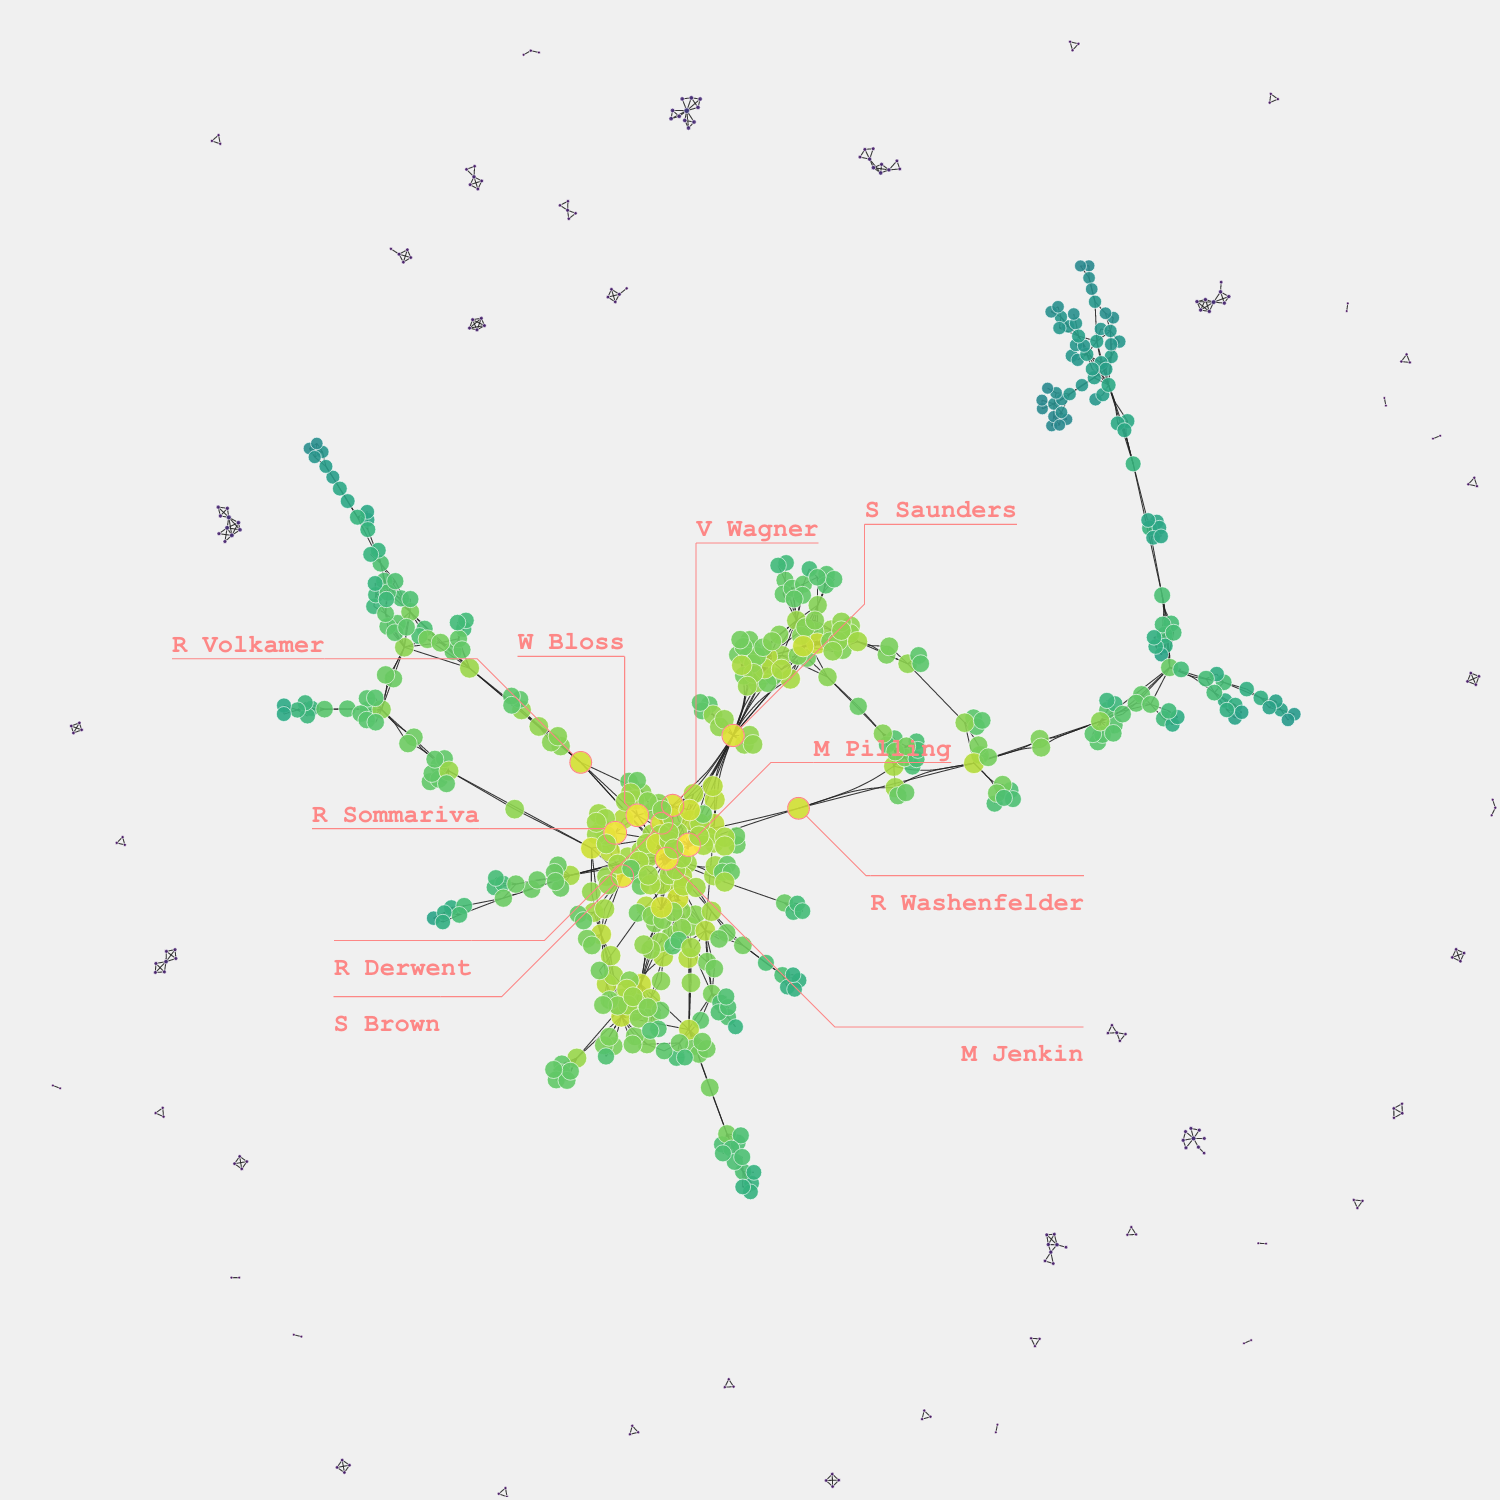
\includegraphics[width=.8\textwidth]{figures_c3/closenessauthor.png}
         
         \begin{table}[H] \centering\begin{tabular}{lr}
\toprule
      \hphantom{ } M Pilling &  0.149995 \\
       \hphantom{ } M Jenkin &  0.146532 \\
    \hphantom{ } R Sommariva &  0.145251 \\
        \hphantom{ } W Bloss &  0.144052 \\
        \hphantom{ } S Brown &  0.142059 \\
     \hphantom{ } S Saunders &  0.140176 \\
       \hphantom{ } V Wagner &  0.139281 \\
      \hphantom{ } R Derwent &  0.136450 \\
     \hphantom{ } R Volkamer &  0.136184 \\
 \hphantom{ } R Washenfelder &  0.135918 \\
\bottomrule
\end{tabular}

    \label{tab:closeness_Author}
    % \caption{\textbf{Author network}: Top 10 ranked items using closeness centrality}
    \end{table}

    
        \caption{ \textbf{Closeness centrality within the co-Author network.} Here a colour/size gradient is seen, with the nodes that are more central (in location) and better connected having a higher closeness than those in the peripheries - which are harder to get to.}
        \label{fig:closeauth}
\end{figure}
% 
% \begin{table}[H]
     \begin{tabular}{p{0.5\textwidth}p{0.35\textwidth}c}
     \toprule
      & & \\\\
     Protocol for the development of the Master Chemical Mechanism, MCM v3 Part A tropospheric degradation of nonaromatic volatile organic compounds & \cite{closeness0} & 0.67  \\ \\
        Protocol for the development of the Master Chemical Mechanism, MCM v3 Part B tropospheric degradation of aromatic volatile organic compounds & \cite{closeness1} & 0.53  \\ \\
        Photochemical ozone creation potentials for organic compounds in northwest Europe calculated with a master chemical mechanism & \cite{closeness2} & 0.45  \\ \\
        World Wide Web site of a Master Chemical Mechanism MCM for use in tropospheric chemistry models & \cite{closeness3} & 0.43  \\ \\
        Photochemical ozone creation potentials for oxygenated volatile organic compounds sensitivity... & \cite{closeness4} & 0.40  \\ \\
        \bottomrule
    \end{tabular}
    \label{tab:closeness_Citation}
    \caption{\textbf{Citation network}: Top 5 ranked items using closeness centrality}
    \end{table}

    
% \begin{table}[H]
     \begin{tabular}{p{0.5\textwidth}p{0.35\textwidth}c}
     \toprule
      & & \\\\
     Protocol for the development of the Master Chemical Mechanism, MCM v3 Part A tropospheric degradation of nonaromatic volatile organic compounds & \cite{closeness0} & 0.80  \\ \\
        Protocol for the development of the Master Chemical Mechanism, MCM v3 Part B tropospheric degradation of aromatic volatile organic compounds & \cite{closeness1} & 0.68  \\ \\
        Atmospheric oxidation capacity sustained by a tropical forest & \cite{closeness2} & 0.61  \\ \\
        Development of a detailed chemical mechanism MCMv3. 1 for the atmospheric oxidation of aromatic hydrocarbons & \cite{closeness3} & 0.61  \\ \\
        HO x radical regeneration in the oxidation of isoprene & \cite{closeness4} & 0.60  \\ \\
        \bottomrule
    \end{tabular}
    \label{tab:closeness_Co-Citation}
    \caption{\textbf{Co-Citation network}: Top 5 ranked items using closeness centrality}
    \end{table}

    
\subsection{Betweenness}
In social networks, it is often important not only to know who has the greatest reach (closeness centrality) but also where bottlenecks or `broker' positions occur. Nodes with a high betweenness control, or limit, the amount of information that can be transferred across the network. If a node lies on a geodesic (the shortest path between two other nodes), we may consider it a `pivotal' node, due to its role within the network \citep{neoj4}. Should such a node then be removed, the overall flow of information incurs either a deviation, the information will either need to travel a longer (alternative) route or may not be able to reach its destination at all \citep{betweenness, between, betweenfast,examples_centrality}.
Betweenness centrality is a count of the number of geodesics which pass through a node. If multiple `shortest' paths are possible, this is accounted for within the denominator. 


\begin{quote}
\textit{
\textbf{Example analogy:} Expanding on the UK rail network analogy, Shrewsbury station serves the critical role of connecting many lines from England to Wales. In removing this station, routes from the Liverpool or Manchester to Cardiff will be greatly increased. Additionally, the Aberystwyth section of the line will then become isolated from the rest of the country.
}
\end{quote}

Authors with a high betweenness in \autoref{fig:betauth} are seen to lie along the joints between clusters. Here we can imagine that removing Li, Griffin or Liu can disrupt the overall flow of collaboration, potentially isolating the work of the Max Planck from that of everyone else. Similarly, Jenkin and Pilling can be seen as holding much of the Leeds cluster together. In removing them from the network (if for example, the refused to collaborate) it is possible to see how many of groups within the Leeds environment may not have worked together, with the cluster potentially separating into several smaller groups. Finally, we see Saunders (Australia), who served to introduce the MCM to the Chinese atmospheric community. In removing her from the network, it can be seen that much of the collaboration which exists would have been significantly less likely.  

\begin{figure}[H]
     \centering
         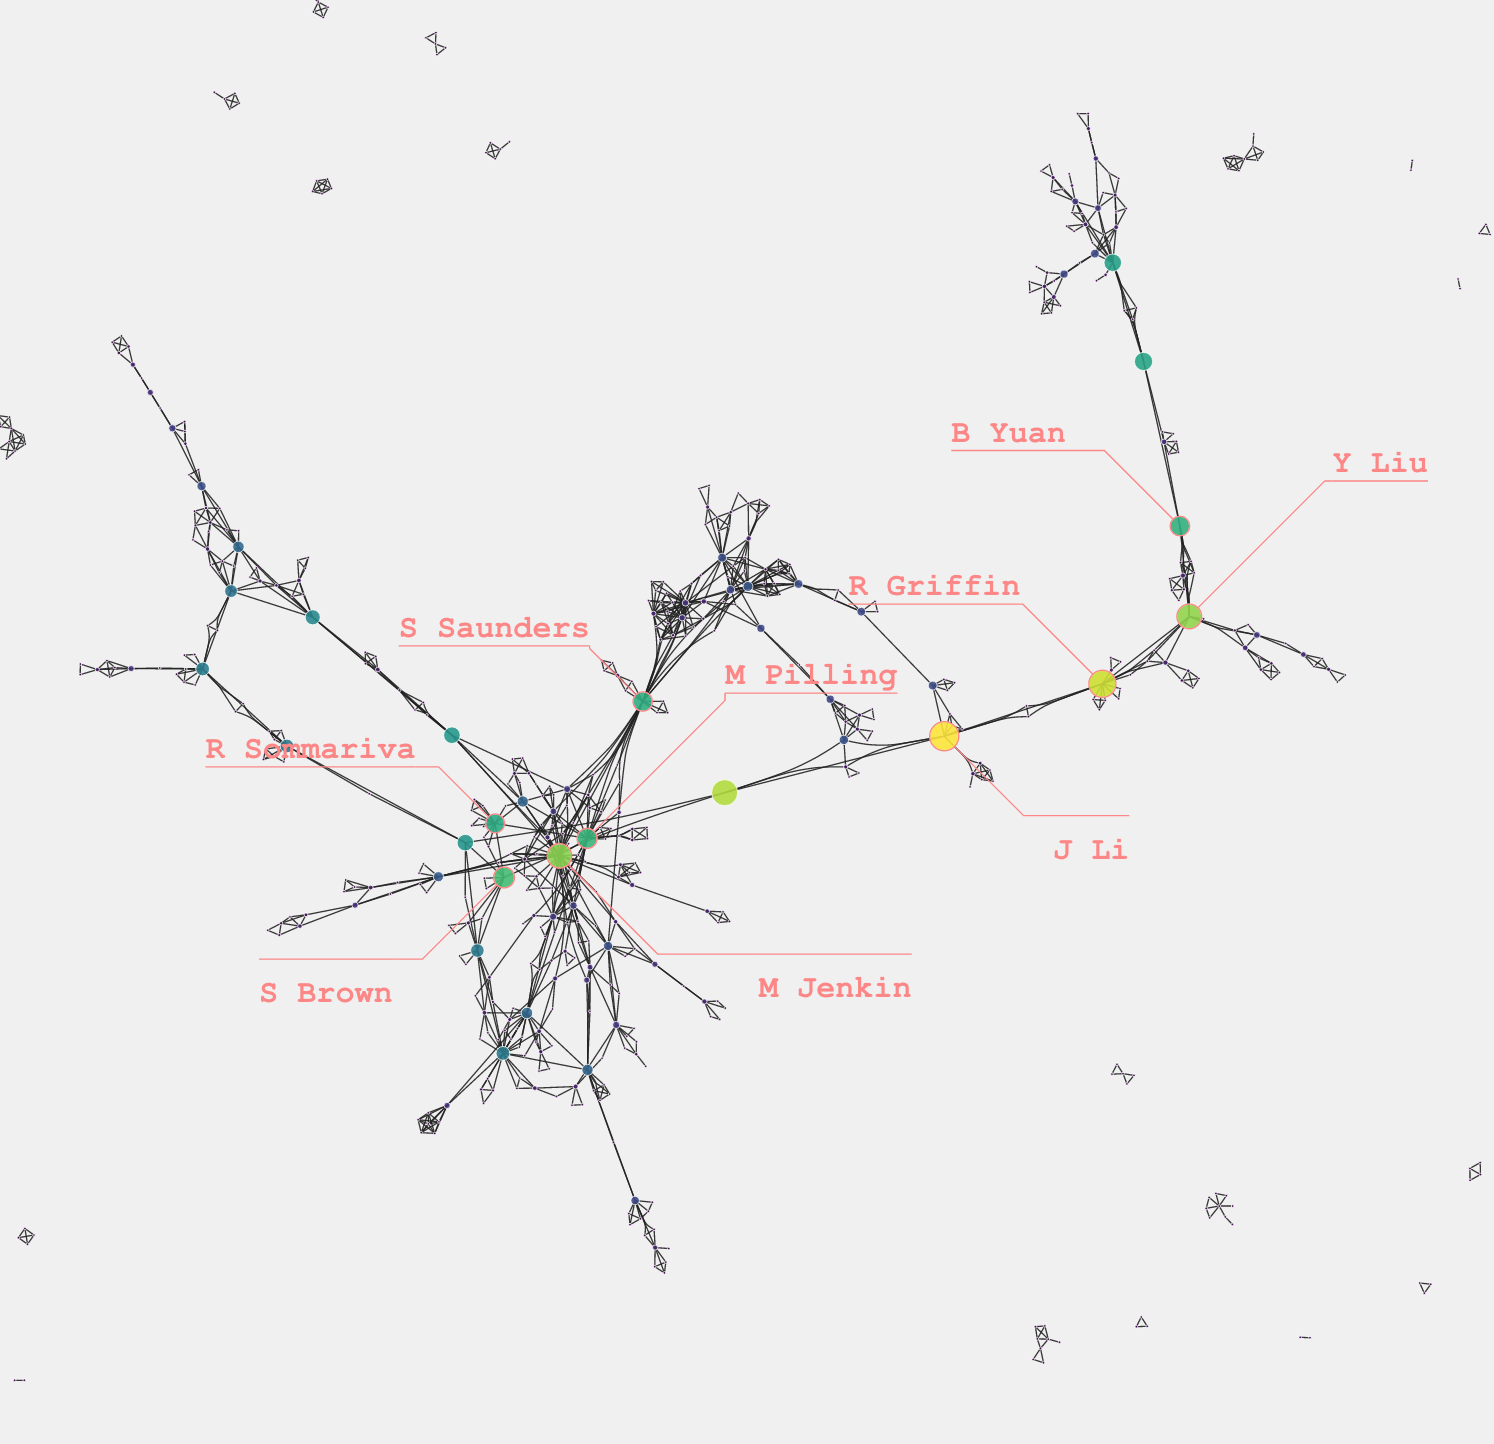
\includegraphics[width=.8\textwidth]{figures_c3/betweenauthor.png}
         \begin{table}[H] \centering\begin{tabular}{lr}
\toprule
           \hphantom{ } J Li &  0.180998 \\
      \hphantom{ } R Griffin &  0.162558 \\
 \hphantom{ } R Washenfelder &  0.153024 \\
          \hphantom{ } Y Liu &  0.142194 \\
       \hphantom{ } M Jenkin &  0.139818 \\
        \hphantom{ } S Brown &  0.110188 \\
      \hphantom{ } M Pilling &  0.102816 \\
         \hphantom{ } B Yuan &  0.099914 \\
     \hphantom{ } S Saunders &  0.097255 \\
    \hphantom{ } R Sommariva &  0.094757 \\
\bottomrule
\end{tabular}

    \label{tab:betweenness_Author}
    % \caption{\textbf{Author network}: Top 10 ranked items using betweenness centrality}
    \end{table}

    
        \caption{ \textbf{Betweenness centrality within the co-Author network.} Nodes which lie on a pivotal position (connecting/bottleneck) tend to have a high betweenness value due to their crutial role within the network.}
        \label{fig:betauth}
\end{figure}


% 
% \begin{table}[H]
     \begin{tabular}{p{0.5\textwidth}p{0.35\textwidth}c}
     \toprule
      & & \\\\
     Impacts of mechanistic changes on HOx formation and recycling in the oxidation of isoprene & \cite{betweenness0} & 0.01  \\ \\
        Protocol for the development of the Master Chemical Mechanism, MCM v3 Part A tropospheric degradation of nonaromatic volatile organic compounds & \cite{betweenness1} & 0.01  \\ \\
        The regional atmospheric chemistry mechanism, version 2 & \cite{betweenness2} & 0.01  \\ \\
        Evaluation of and pinene degradation in the detailed tropospheric chemistry mechanism, MCM v3. 1, using environmental chamber data & \cite{betweenness3} & 0.01  \\ \\
        A review of tropospheric atmospheric chemistry and gasphase chemical mechanisms for air quality modeling & \cite{betweenness4} & 0.01  \\ \\
        \bottomrule
    \end{tabular}
    \label{tab:betweenness_Citation}
    \caption{\textbf{Citation network}: Top 5 ranked items using betweenness centrality}
    \end{table}

    
% \begin{table}[H]
     \begin{tabular}{p{0.5\textwidth}p{0.35\textwidth}c}
     \toprule
      & & \\\\
     Protocol for the development of the Master Chemical Mechanism, MCM v3 Part A tropospheric degradation of nonaromatic volatile organic compounds & \cite{betweenness0} & 0.12  \\ \\
        Protocol for the development of the Master Chemical Mechanism, MCM v3 Part B tropospheric degradation of aromatic volatile organic compounds & \cite{betweenness1} & 0.10  \\ \\
        HO x radical regeneration in the oxidation of isoprene & \cite{betweenness2} & 0.05  \\ \\
        The MCM v3. 3.1 degradation scheme for isoprene & \cite{betweenness3} & 0.04  \\ \\
        Development of a detailed chemical mechanism MCMv3. 1 for the atmospheric oxidation of aromatic hydrocarbons & \cite{betweenness4} & 0.04  \\ \\
        \bottomrule
    \end{tabular}
    \label{tab:betweenness_Co-Citation}
    \caption{\textbf{Co-Citation network}: Top 5 ranked items using betweenness centrality}
    \end{table}

    
\subsection{Spectral methods and matrix analysis}

Graphs can often be represented in the form of relationship (adjacency) matrixes (ref Chapter 1). This allows us to apply the theory of linear maps, such as eigenvectors and values, to stochiometric data in matrix form. Such methods have been around since the 1950s, \citep{seeley}, but mainly became popular with the release of Larry Page's page-rank algorithm \citep{google} - the algorithm that began google. These methods, in addition to the HITS algorithm \autoref{hits}, make use of a graphs native matrix representation to calculate node importance. Spectral algorithms can be broken down into four categories \citep{spectral}:

\begin{table}[H]
  \centering
\begin{tabular}{p{.6\textwidth}||p{.26\textwidth} p{.26\textwidth}}
\hline
 & No Normalisation  & Row Normalisation \\
 \hline \hline
No Damping & Eigenvector \citep{eigen, eigen2}  \: & Markov Chain Steady State \citep{seeley} \: \\
Damping & Katz \citep{katz} \: & Total Effect Centrality PageRank \citep{google} \\ \hline
\end{tabular}
\end{table}


Here damping terms represent the probability of moving to the new random starting position, allowing for the user to `randomly select a new webpage' or leave an isolated cluster. The normalisation of the matrix does not affect the node ranking, but merely adjusts the numerical output of the algorithm. It is for this reason that its overall practicality may be debated \citep{spectral}. Since page rank is the most common of these methods and allows for a tune-able degree of randomness within network propagation. This is discussed in more detail in the next subsection.


    
    \paragraph*{Hypertext Induced Topic Search (HITS)}\label{hits}
    A common eigenvector algorithm used for classifying webpages is the 
    HITS algorithm. This helps categorise the role of a node as either a Hub or an Authority,
     \citep{hits,hitsvspagerank,hitsweb}. Similar to the in and out-degree metrics, this algorithm separates nodes with many outgoing links (an authority) from those with many ingoing ones (an information hub). Overall this provides similar results to the in/out degree, although since it looks more on how information propagates across the network as a whole, it often provides more accurate, and different, rankings to simple degree analysis.  
     
     
% \begin{table}[H]
     \begin{tabular}{p{0.5\textwidth}p{0.35\textwidth}c}
     \toprule
      & & \\\\
     A Common Representative Intermediates CRI mechanism for VOC degradation. Part 3 Development of a secondary organic aerosol module & \cite{Hub0} & 0.01  \\ \\
        HOx budgets during HOxComp A case study of HOx chemistry under NOxlimited conditions & \cite{Hub1} & 0.01  \\ \\
        Detailed chemical analysis of regionalscale air pollution in western Portugal using an adapted version of MCM v3. 1 & \cite{Hub2} & 0.01  \\ \\
        Box model studies of the secondary organic aerosol formation under different HCNOx conditions using the subset of the Master Chemical Mechanism for pinene & \cite{Hub3} & 0.01  \\ \\
        Reporting the sensitivity of laserinduced fluorescence instruments used for HO2 detection to an interference from RO2 radicals and introducing a novel approach that & \cite{Hub4} & 0.01  \\ \\
        \bottomrule
    \end{tabular}
    \label{tab:Hub_Citation}
    \caption{\textbf{Citation network}: Top 5 ranked items using Hub centrality}
    \end{table}

    
% \begin{table}[H]
     \begin{tabular}{p{0.5\textwidth}p{0.35\textwidth}c}
     \toprule
      & & \\\\
     Protocol for the development of the Master Chemical Mechanism, MCM v3 Part A tropospheric degradation of nonaromatic volatile organic compounds & \cite{Authority0} & 0.11  \\ \\
        Protocol for the development of the Master Chemical Mechanism, MCM v3 Part B tropospheric degradation of aromatic volatile organic compounds & \cite{Authority1} & 0.07  \\ \\
        Development of a detailed chemical mechanism MCMv3. 1 for the atmospheric oxidation of aromatic hydrocarbons & \cite{Authority2} & 0.04  \\ \\
        Atmospheric oxidation capacity sustained by a tropical forest & \cite{Authority3} & 0.02  \\ \\
        Photochemical ozone creation potentials for organic compounds in northwest Europe calculated with a master chemical mechanism & \cite{Authority4} & 0.02  \\ \\
        \bottomrule
    \end{tabular}
    \label{tab:Authority_Citation}
    \caption{\textbf{Citation network}: Top 5 ranked items using Authority centrality}
    \end{table}

    






\subsection{Page Rank}
Arguably the best-known centrality algorithm is PageRank. This is a spectral method for measuring the transitive influence of a node, by taking the effect of neighbours and by their neighbours into account \citep{neoj4}. The page rank algorithm was initially developed to provide a better way of ranking web pages \citep{google}- here an important page is not only one of many links, but links to other important sources. In the context of academic papers, that same paper also found that in predicting future citations, the page rank algorithm fared better than using the current citation count of a paper. 
To explain how this works, we will look at the mathematics behind the algorithm, and then eventually apply it to the co-authorship graph in \autoref{sec:applypr}

\paragraph{The Google Matrix}
To solve for page rank, a google matrix must first be constructed. Once done this is iterated until convergence is reached. 

To build a google matrix, we must first generate a dyadic link map of the graph\footnote{In sociology a dyad is a group of two people - the smallest possible social group.} - its adjacency matrix $A_{i,j}$ ($i,j$ are the source target indexes). This is then converted into a Markov matrix $M_{i.j}$ by dividing each column $j$ by the sum of the total outgoing links of node $j$, Algorithm \ref{eqn:markov}.
Species with no outgoing links (sinks), are adjusted with either a personalised list of values or the constant $1/n$, (where $n$ is the number of nodes) to replace the zero-sum columns. This produces a normalised\footnote{ \: $\Sigma_{i=1,n} M(i,j) = $ unity} matrix of Markov chains representing the fractional production for node $j$ from all other nodes.

\begin{algorithm} \caption{Adjacency to Markov matrix.}
\begin{algorithmic}[1]
\State Obtain graph adjacency matrix, $A_{i,j}$.
\Repeat
\ForEach{$ j \in \mathcal{}$ columns}
\State $M($:$,j) \gets A($:$,j) / \Sigma_{i=1,n} A(j,i)$
\EndFor
\Until {$\Sigma_{i=1,n} M(i,j) = 1$}

\end{algorithmic}\label{eqn:markov}
\end{algorithm}



The google matrix $G_{i,j}$ can now be defined using \autoref{eqn:google}.
 Cyclic reactions and nodes that only point towards each other within a group can `trap' the user, increasing their ranks. 
 To account for this, a damping factor, typically $\beta = 0.85$, is used. This defines the probability that the user follows a link, and that for which they randomly select another page: $(1-\beta)$ \footnote{Also known as teleportation.}. The damping factor used varies greatly with the application, with values such as $\beta = 0.694$ having been found optimal for the use of biological data \citep{biopr}.


\begin{center}
\begin{equation}
     G_{i,j} = \beta M + \cfrac{1 - \beta}{n}
 %\vec{dsfds}
 \label{eqn:google}
\end{equation}
\begin{tabular}{ccl}
$\beta$&-&\textit{Probability the user follows a link} \\
 $(1 - \beta)$&-&\textit{Probability the user does not follow a link (teleportation)} \\
$n$&-&\textit{Number of items / species}\\
$M$&-&\textit{Normalised markov matrix}
\end{tabular}
\end{center}


\paragraph{Solving the algebra}

Once defined, the google matrix is solved by propagating a one's vector, $r$ of length $n$, where $n$ is the number of species using Algorithm \ref{eqn:forwards}.


\begin{algorithm} \caption{Solving the google matrix linear algebra}
\begin{algorithmic}[1]
\State {Define value vectors $\Bar{r}_t$ and $\Bar{r}_{t+1}$:}
\State  $\Bar{r}_t \:\:= [1_1, 1_2, ... , 1_n]$, $\Bar{r}_{t+1} = [0_1, 0_2, ... , 0_n]$
\State
\While {$||\Bar{r}_{t+1} - \Bar{r}_t|| > \epsilon$}
\State $\Bar{r}_{t+1} \gets M . \Bar{r}_t$
\State $\Bar{r}_t = \Bar{r}_{t+1}$
\EndWhile
\end{algorithmic}\label{eqn:forwards}
\end{algorithm}


 This is repeated until a pre-defined tolerance, $\epsilon$ is reached. For best results, this can be set to just under the numerical precision of the programming language/hardware. 


For smaller systems, it is possible to use the LAPACK \citep{lapack} library, as used by \citep{numpy}. For a large network, however, the computation of an $n \times n $ matrix can be very memory inefficient for small machines. It is then possible to apply the methods as described above using a sparse matrix on per-node bases as can be seen within the scipy implementation of the networkx source code \citep{scipy,networkx}.

\paragraph{Prediction}\label{sec:applypr}
As the PageRank algorithm is a physical representation looking at how quantities `flow' within a network, it can be used to identify not only the bottlenecks (betweenness centrality) but also any nodes which are connected well within the network. As the flows between a node are somewhat governed by the number of links it contains, the PageRank algorithms tend to correlate, but not a dependance, on the betweenness of a node. \autoref{fig:pagerankauth} shows the PageRank algorithm to identify important authors within each `cluster' or research group. Due to its propagating nature authors connected to these important nodes are often also of greater importance. An application of this can again be the determination of how to best spread new results or information with the least number of people. \textit{Note: if we only had one person we would probably use the node with the highest closeness centrality.}

\begin{figure}[H]
     \centering
         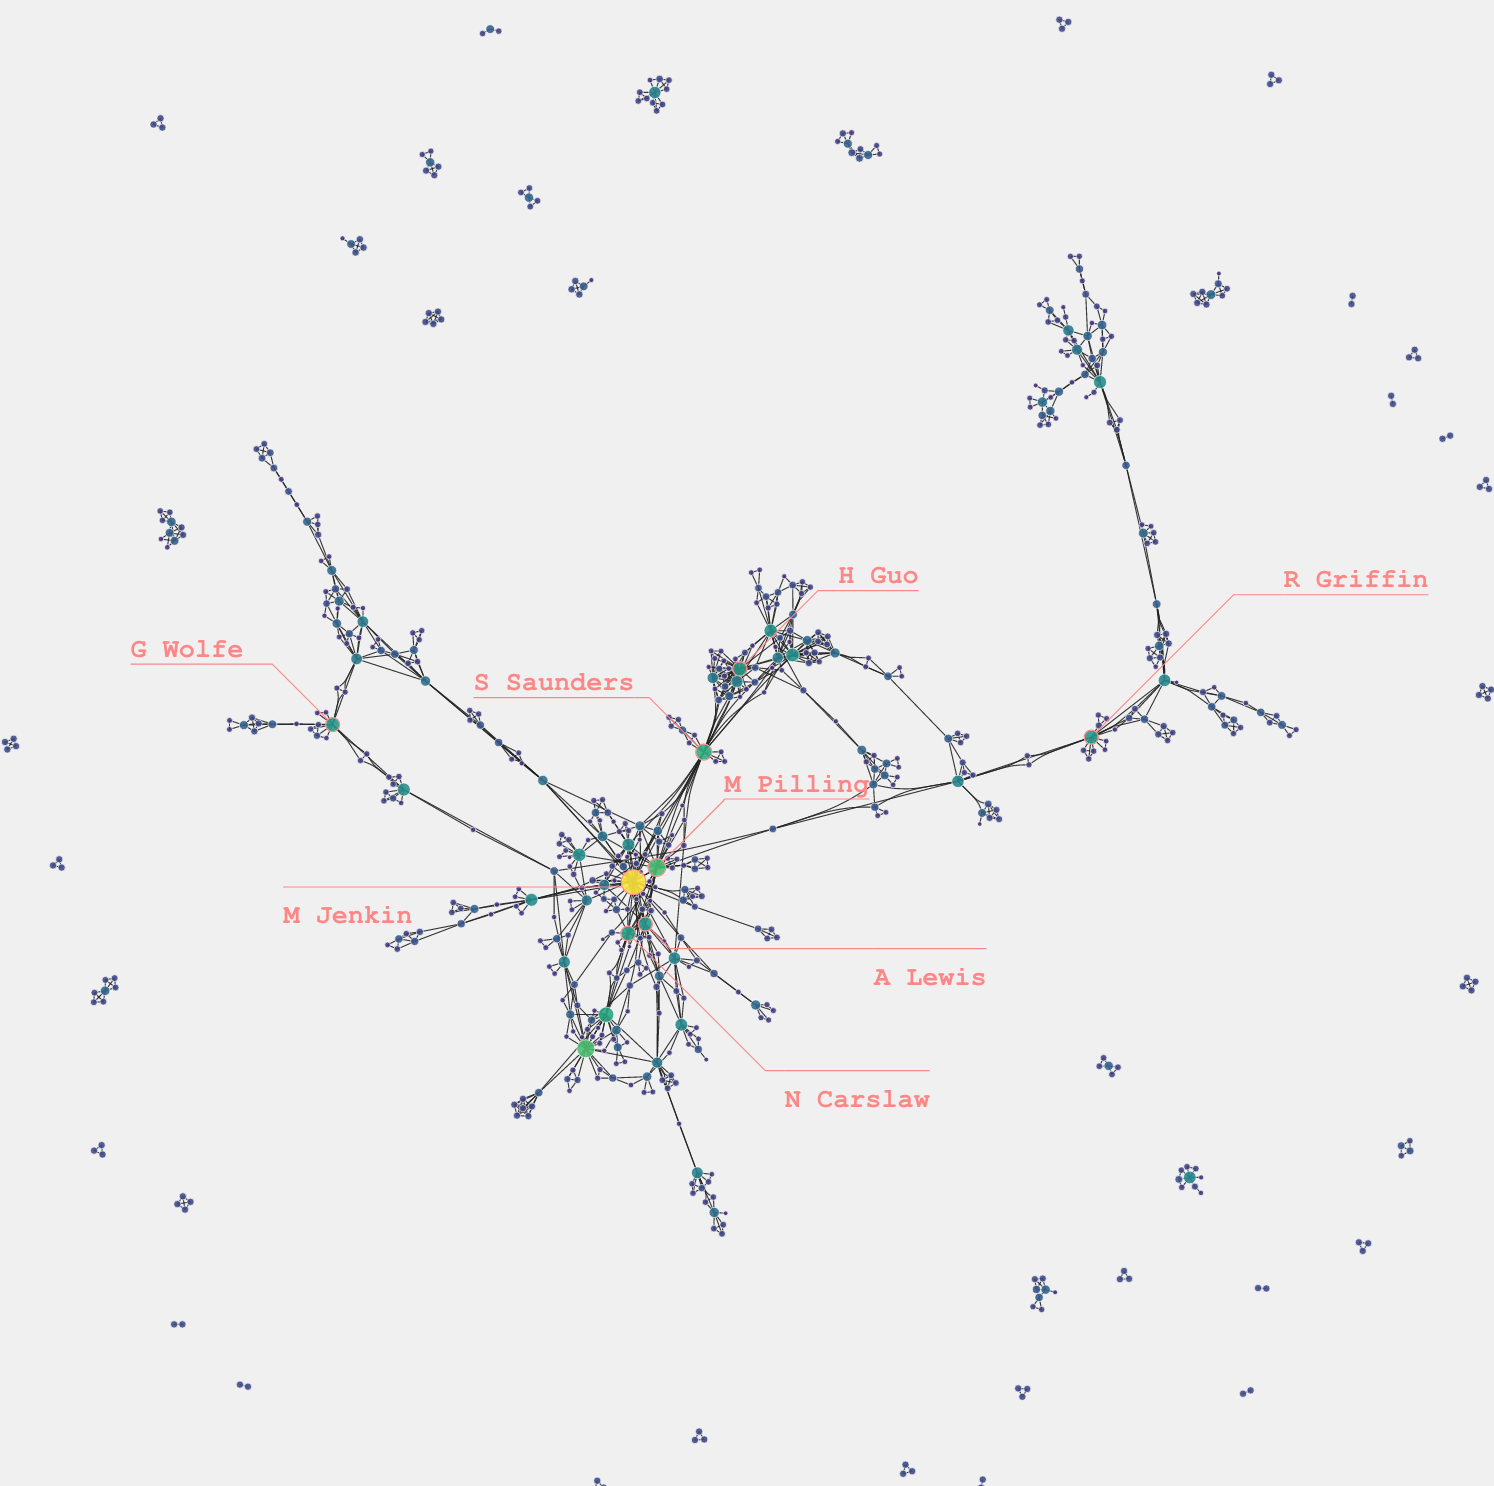
\includegraphics[width=.8\textwidth]{figures_c3/pagerankauthor.png}

        \begin{table}[H] \centering\begin{tabular}{lr}
\toprule
   \hphantom{ } M Jenkin &  0.010435 \\
  \hphantom{ } L Whalley &  0.006589 \\
  \hphantom{ } M Pilling &  0.006488 \\
 \hphantom{ } S Saunders &  0.005591 \\
    \hphantom{ } D Heard &  0.005192 \\
  \hphantom{ } N Carslaw &  0.004833 \\
      \hphantom{ } H Guo &  0.004594 \\
    \hphantom{ } G Wolfe &  0.004523 \\
    \hphantom{ } A Lewis &  0.004508 \\
  \hphantom{ } R Griffin &  0.004500 \\
\bottomrule
\end{tabular}

    \label{tab:pagerank_Author}

    \end{table}

    
                \caption{ \textbf{Page Rank centrality within the co-Author network}.}
        \label{fig:pagerankauth}
\end{figure}


\subsubsection{Conclusions}
In this section, we have explored the use of centrality metrics to provide us with information on an unweighted co-authorship network of the MCM. Having used these to demonstrate the different roles that may be extracted from a node, we can move on to applying them to a chemical mechanism. In the next section, a global set of metrics will be used to determine the network type/structure of the MCM. Once this has been done, graph construction using simulation results (a weighted graph) will be looked into in \autoref{sec:graphconstruction}. 
% 
% 
% \begin{table}[H]
     \begin{tabular}{p{0.5\textwidth}p{0.35\textwidth}c}
     \toprule
      & & \\\\
     World Wide Web site of a Master Chemical Mechanism MCM for use in tropospheric chemistry models & \cite{pagerank0} & 0.09  \\ \\
        Protocol for the development of the Master Chemical Mechanism, MCM v3 Part A tropospheric degradation of nonaromatic volatile organic compounds & \cite{pagerank1} & 0.07  \\ \\
        Photochemical ozone creation potentials for organic compounds in northwest Europe calculated with a master chemical mechanism & \cite{pagerank2} & 0.07  \\ \\
        Protocol for the development of the Master Chemical Mechanism, MCM v3 Part B tropospheric degradation of aromatic volatile organic compounds & \cite{pagerank3} & 0.05  \\ \\
        Modeling OH, HO2, and RO2 radicals in the marine boundary layer 2. Mechanism reduction and... & \cite{pagerank4} & 0.03  \\ \\
        \bottomrule
    \end{tabular}
    \label{tab:pagerank_Citation}
    \caption{\textbf{Citation network}: Top 5 ranked items using pagerank centrality}
    \end{table}

    
% \begin{table}[H]
     \begin{tabular}{p{0.5\textwidth}p{0.35\textwidth}c}
     \toprule
      & & \\\\
     Protocol for the development of the Master Chemical Mechanism, MCM v3 Part A tropospheric degradation of nonaromatic volatile organic compounds & \cite{pagerank0} & 0.06  \\ \\
        Protocol for the development of the Master Chemical Mechanism, MCM v3 Part B tropospheric degradation of aromatic volatile organic compounds & \cite{pagerank1} & 0.03  \\ \\
        Atmospheric oxidation capacity sustained by a tropical forest & \cite{pagerank2} & 0.03  \\ \\
        Development of a detailed chemical mechanism MCMv3. 1 for the atmospheric oxidation of aromatic hydrocarbons & \cite{pagerank3} & 0.02  \\ \\
        HO x radical regeneration in the oxidation of isoprene & \cite{pagerank4} & 0.02  \\ \\
        \bottomrule
    \end{tabular}
    \label{tab:pagerank_Co-Citation}
    \caption{\textbf{Co-Citation network}: Top 5 ranked items using pagerank centrality}
    \end{table}

    
